% Options for packages loaded elsewhere
\PassOptionsToPackage{unicode}{hyperref}
\PassOptionsToPackage{hyphens}{url}
\PassOptionsToPackage{dvipsnames,svgnames,x11names}{xcolor}
%
\documentclass[
  letterpaper,
  DIV=11,
  numbers=noendperiod]{scrartcl}

\usepackage{amsmath,amssymb}
\usepackage{iftex}
\ifPDFTeX
  \usepackage[T1]{fontenc}
  \usepackage[utf8]{inputenc}
  \usepackage{textcomp} % provide euro and other symbols
\else % if luatex or xetex
  \usepackage{unicode-math}
  \defaultfontfeatures{Scale=MatchLowercase}
  \defaultfontfeatures[\rmfamily]{Ligatures=TeX,Scale=1}
\fi
\usepackage{lmodern}
\ifPDFTeX\else  
    % xetex/luatex font selection
\fi
% Use upquote if available, for straight quotes in verbatim environments
\IfFileExists{upquote.sty}{\usepackage{upquote}}{}
\IfFileExists{microtype.sty}{% use microtype if available
  \usepackage[]{microtype}
  \UseMicrotypeSet[protrusion]{basicmath} % disable protrusion for tt fonts
}{}
\makeatletter
\@ifundefined{KOMAClassName}{% if non-KOMA class
  \IfFileExists{parskip.sty}{%
    \usepackage{parskip}
  }{% else
    \setlength{\parindent}{0pt}
    \setlength{\parskip}{6pt plus 2pt minus 1pt}}
}{% if KOMA class
  \KOMAoptions{parskip=half}}
\makeatother
\usepackage{xcolor}
\setlength{\emergencystretch}{3em} % prevent overfull lines
\setcounter{secnumdepth}{-\maxdimen} % remove section numbering
% Make \paragraph and \subparagraph free-standing
\ifx\paragraph\undefined\else
  \let\oldparagraph\paragraph
  \renewcommand{\paragraph}[1]{\oldparagraph{#1}\mbox{}}
\fi
\ifx\subparagraph\undefined\else
  \let\oldsubparagraph\subparagraph
  \renewcommand{\subparagraph}[1]{\oldsubparagraph{#1}\mbox{}}
\fi

\usepackage{color}
\usepackage{fancyvrb}
\newcommand{\VerbBar}{|}
\newcommand{\VERB}{\Verb[commandchars=\\\{\}]}
\DefineVerbatimEnvironment{Highlighting}{Verbatim}{commandchars=\\\{\}}
% Add ',fontsize=\small' for more characters per line
\usepackage{framed}
\definecolor{shadecolor}{RGB}{241,243,245}
\newenvironment{Shaded}{\begin{snugshade}}{\end{snugshade}}
\newcommand{\AlertTok}[1]{\textcolor[rgb]{0.68,0.00,0.00}{#1}}
\newcommand{\AnnotationTok}[1]{\textcolor[rgb]{0.37,0.37,0.37}{#1}}
\newcommand{\AttributeTok}[1]{\textcolor[rgb]{0.40,0.45,0.13}{#1}}
\newcommand{\BaseNTok}[1]{\textcolor[rgb]{0.68,0.00,0.00}{#1}}
\newcommand{\BuiltInTok}[1]{\textcolor[rgb]{0.00,0.23,0.31}{#1}}
\newcommand{\CharTok}[1]{\textcolor[rgb]{0.13,0.47,0.30}{#1}}
\newcommand{\CommentTok}[1]{\textcolor[rgb]{0.37,0.37,0.37}{#1}}
\newcommand{\CommentVarTok}[1]{\textcolor[rgb]{0.37,0.37,0.37}{\textit{#1}}}
\newcommand{\ConstantTok}[1]{\textcolor[rgb]{0.56,0.35,0.01}{#1}}
\newcommand{\ControlFlowTok}[1]{\textcolor[rgb]{0.00,0.23,0.31}{#1}}
\newcommand{\DataTypeTok}[1]{\textcolor[rgb]{0.68,0.00,0.00}{#1}}
\newcommand{\DecValTok}[1]{\textcolor[rgb]{0.68,0.00,0.00}{#1}}
\newcommand{\DocumentationTok}[1]{\textcolor[rgb]{0.37,0.37,0.37}{\textit{#1}}}
\newcommand{\ErrorTok}[1]{\textcolor[rgb]{0.68,0.00,0.00}{#1}}
\newcommand{\ExtensionTok}[1]{\textcolor[rgb]{0.00,0.23,0.31}{#1}}
\newcommand{\FloatTok}[1]{\textcolor[rgb]{0.68,0.00,0.00}{#1}}
\newcommand{\FunctionTok}[1]{\textcolor[rgb]{0.28,0.35,0.67}{#1}}
\newcommand{\ImportTok}[1]{\textcolor[rgb]{0.00,0.46,0.62}{#1}}
\newcommand{\InformationTok}[1]{\textcolor[rgb]{0.37,0.37,0.37}{#1}}
\newcommand{\KeywordTok}[1]{\textcolor[rgb]{0.00,0.23,0.31}{#1}}
\newcommand{\NormalTok}[1]{\textcolor[rgb]{0.00,0.23,0.31}{#1}}
\newcommand{\OperatorTok}[1]{\textcolor[rgb]{0.37,0.37,0.37}{#1}}
\newcommand{\OtherTok}[1]{\textcolor[rgb]{0.00,0.23,0.31}{#1}}
\newcommand{\PreprocessorTok}[1]{\textcolor[rgb]{0.68,0.00,0.00}{#1}}
\newcommand{\RegionMarkerTok}[1]{\textcolor[rgb]{0.00,0.23,0.31}{#1}}
\newcommand{\SpecialCharTok}[1]{\textcolor[rgb]{0.37,0.37,0.37}{#1}}
\newcommand{\SpecialStringTok}[1]{\textcolor[rgb]{0.13,0.47,0.30}{#1}}
\newcommand{\StringTok}[1]{\textcolor[rgb]{0.13,0.47,0.30}{#1}}
\newcommand{\VariableTok}[1]{\textcolor[rgb]{0.07,0.07,0.07}{#1}}
\newcommand{\VerbatimStringTok}[1]{\textcolor[rgb]{0.13,0.47,0.30}{#1}}
\newcommand{\WarningTok}[1]{\textcolor[rgb]{0.37,0.37,0.37}{\textit{#1}}}

\providecommand{\tightlist}{%
  \setlength{\itemsep}{0pt}\setlength{\parskip}{0pt}}\usepackage{longtable,booktabs,array}
\usepackage{calc} % for calculating minipage widths
% Correct order of tables after \paragraph or \subparagraph
\usepackage{etoolbox}
\makeatletter
\patchcmd\longtable{\par}{\if@noskipsec\mbox{}\fi\par}{}{}
\makeatother
% Allow footnotes in longtable head/foot
\IfFileExists{footnotehyper.sty}{\usepackage{footnotehyper}}{\usepackage{footnote}}
\makesavenoteenv{longtable}
\usepackage{graphicx}
\makeatletter
\def\maxwidth{\ifdim\Gin@nat@width>\linewidth\linewidth\else\Gin@nat@width\fi}
\def\maxheight{\ifdim\Gin@nat@height>\textheight\textheight\else\Gin@nat@height\fi}
\makeatother
% Scale images if necessary, so that they will not overflow the page
% margins by default, and it is still possible to overwrite the defaults
% using explicit options in \includegraphics[width, height, ...]{}
\setkeys{Gin}{width=\maxwidth,height=\maxheight,keepaspectratio}
% Set default figure placement to htbp
\makeatletter
\def\fps@figure{htbp}
\makeatother

\KOMAoption{captions}{tableheading}
\makeatletter
\makeatother
\makeatletter
\makeatother
\makeatletter
\@ifpackageloaded{caption}{}{\usepackage{caption}}
\AtBeginDocument{%
\ifdefined\contentsname
  \renewcommand*\contentsname{Table of contents}
\else
  \newcommand\contentsname{Table of contents}
\fi
\ifdefined\listfigurename
  \renewcommand*\listfigurename{List of Figures}
\else
  \newcommand\listfigurename{List of Figures}
\fi
\ifdefined\listtablename
  \renewcommand*\listtablename{List of Tables}
\else
  \newcommand\listtablename{List of Tables}
\fi
\ifdefined\figurename
  \renewcommand*\figurename{Figure}
\else
  \newcommand\figurename{Figure}
\fi
\ifdefined\tablename
  \renewcommand*\tablename{Table}
\else
  \newcommand\tablename{Table}
\fi
}
\@ifpackageloaded{float}{}{\usepackage{float}}
\floatstyle{ruled}
\@ifundefined{c@chapter}{\newfloat{codelisting}{h}{lop}}{\newfloat{codelisting}{h}{lop}[chapter]}
\floatname{codelisting}{Listing}
\newcommand*\listoflistings{\listof{codelisting}{List of Listings}}
\makeatother
\makeatletter
\@ifpackageloaded{caption}{}{\usepackage{caption}}
\@ifpackageloaded{subcaption}{}{\usepackage{subcaption}}
\makeatother
\makeatletter
\@ifpackageloaded{tcolorbox}{}{\usepackage[skins,breakable]{tcolorbox}}
\makeatother
\makeatletter
\@ifundefined{shadecolor}{\definecolor{shadecolor}{rgb}{.97, .97, .97}}
\makeatother
\makeatletter
\makeatother
\makeatletter
\makeatother
\ifLuaTeX
  \usepackage{selnolig}  % disable illegal ligatures
\fi
\IfFileExists{bookmark.sty}{\usepackage{bookmark}}{\usepackage{hyperref}}
\IfFileExists{xurl.sty}{\usepackage{xurl}}{} % add URL line breaks if available
\urlstyle{same} % disable monospaced font for URLs
\hypersetup{
  pdftitle={Class13},
  colorlinks=true,
  linkcolor={blue},
  filecolor={Maroon},
  citecolor={Blue},
  urlcolor={Blue},
  pdfcreator={LaTeX via pandoc}}

\title{Class13}
\author{}
\date{}

\begin{document}
\maketitle
\ifdefined\Shaded\renewenvironment{Shaded}{\begin{tcolorbox}[enhanced, interior hidden, boxrule=0pt, borderline west={3pt}{0pt}{shadecolor}, sharp corners, breakable, frame hidden]}{\end{tcolorbox}}\fi

\begin{Shaded}
\begin{Highlighting}[]
\FunctionTok{library}\NormalTok{(DESeq2)}
\end{Highlighting}
\end{Shaded}

\begin{Shaded}
\begin{Highlighting}[]
\NormalTok{counts }\OtherTok{\textless{}{-}} \FunctionTok{read.csv}\NormalTok{(}\StringTok{"airway\_scaledcounts.csv"}\NormalTok{, }\AttributeTok{row.names=}\DecValTok{1}\NormalTok{)}
\NormalTok{metadata }\OtherTok{\textless{}{-}}  \FunctionTok{read.csv}\NormalTok{(}\StringTok{"airway\_metadata.csv"}\NormalTok{)}
\end{Highlighting}
\end{Shaded}

\begin{quote}
Q1. How many genes are in this dataset?
\end{quote}

\begin{Shaded}
\begin{Highlighting}[]
\FunctionTok{nrow}\NormalTok{(counts)}
\end{Highlighting}
\end{Shaded}

\begin{verbatim}
[1] 38694
\end{verbatim}

\begin{quote}
Q2. How many `control' cell lines do we have?
\end{quote}

\begin{Shaded}
\begin{Highlighting}[]
\FunctionTok{sum}\NormalTok{(metadata}\SpecialCharTok{$}\NormalTok{dex }\SpecialCharTok{==} \StringTok{"control"}\NormalTok{)}
\end{Highlighting}
\end{Shaded}

\begin{verbatim}
[1] 4
\end{verbatim}

\begin{Shaded}
\begin{Highlighting}[]
\NormalTok{metadata}
\end{Highlighting}
\end{Shaded}

\begin{verbatim}
          id     dex celltype     geo_id
1 SRR1039508 control   N61311 GSM1275862
2 SRR1039509 treated   N61311 GSM1275863
3 SRR1039512 control  N052611 GSM1275866
4 SRR1039513 treated  N052611 GSM1275867
5 SRR1039516 control  N080611 GSM1275870
6 SRR1039517 treated  N080611 GSM1275871
7 SRR1039520 control  N061011 GSM1275874
8 SRR1039521 treated  N061011 GSM1275875
\end{verbatim}

I want to compare the control to the treated columns. To do this I will:

-Step 1: Identify and extract the ``control'' columns. -Step 2:
Calculate the mean value per gene for all ``control'' columns, and save
as \texttt{control.mean}. -Step 3: Do the same for ``treated'' columns.
-Step 4: Compare the \texttt{control.mean} and \texttt{treated.mean}.

\begin{Shaded}
\begin{Highlighting}[]
\NormalTok{control.inds }\OtherTok{\textless{}{-}}\NormalTok{ metadata}\SpecialCharTok{$}\NormalTok{dex}\SpecialCharTok{==}\StringTok{"control"}
\end{Highlighting}
\end{Shaded}

\begin{Shaded}
\begin{Highlighting}[]
\NormalTok{metadata[control.inds,]}
\end{Highlighting}
\end{Shaded}

\begin{verbatim}
          id     dex celltype     geo_id
1 SRR1039508 control   N61311 GSM1275862
3 SRR1039512 control  N052611 GSM1275866
5 SRR1039516 control  N080611 GSM1275870
7 SRR1039520 control  N061011 GSM1275874
\end{verbatim}

\begin{Shaded}
\begin{Highlighting}[]
\NormalTok{control.mean }\OtherTok{\textless{}{-}} \FunctionTok{rowMeans}\NormalTok{(counts[,control.inds])}
\FunctionTok{head}\NormalTok{(control.mean)}
\end{Highlighting}
\end{Shaded}

\begin{verbatim}
ENSG00000000003 ENSG00000000005 ENSG00000000419 ENSG00000000457 ENSG00000000460 
         900.75            0.00          520.50          339.75           97.25 
ENSG00000000938 
           0.75 
\end{verbatim}

\begin{quote}
Q3. How would you make the below code in either approach more robust? Is
there a function that could help here?
\end{quote}

\begin{quote}
Q4. Follow the same procedure for the treated samples (i.e.~calculate
the mean per gene across drug treated samples and assign to a labeled
vector called treated.mean)
\end{quote}

\begin{Shaded}
\begin{Highlighting}[]
\NormalTok{treated.inds }\OtherTok{\textless{}{-}}\NormalTok{ metadata}\SpecialCharTok{$}\NormalTok{dex}\SpecialCharTok{==}\StringTok{"treated"}
\end{Highlighting}
\end{Shaded}

\begin{Shaded}
\begin{Highlighting}[]
\NormalTok{metadata[treated.inds,]}
\end{Highlighting}
\end{Shaded}

\begin{verbatim}
          id     dex celltype     geo_id
2 SRR1039509 treated   N61311 GSM1275863
4 SRR1039513 treated  N052611 GSM1275867
6 SRR1039517 treated  N080611 GSM1275871
8 SRR1039521 treated  N061011 GSM1275875
\end{verbatim}

\begin{Shaded}
\begin{Highlighting}[]
\NormalTok{treated.mean }\OtherTok{\textless{}{-}} \FunctionTok{rowMeans}\NormalTok{(counts[,treated.inds])}
\FunctionTok{head}\NormalTok{(treated.mean)}
\end{Highlighting}
\end{Shaded}

\begin{verbatim}
ENSG00000000003 ENSG00000000005 ENSG00000000419 ENSG00000000457 ENSG00000000460 
         658.00            0.00          546.00          316.50           78.75 
ENSG00000000938 
           0.00 
\end{verbatim}

We will combine our meancount data for bookkeeping purposes:

\begin{Shaded}
\begin{Highlighting}[]
\NormalTok{meancounts }\OtherTok{\textless{}{-}} \FunctionTok{data.frame}\NormalTok{(control.mean, treated.mean)}
\end{Highlighting}
\end{Shaded}

Let's see what these count values look like:

\begin{quote}
Q5 (a). Create a scatter plot showing the mean of the treated samples
against the mean of the control samples. Your plot should look something
like the following.
\end{quote}

\begin{Shaded}
\begin{Highlighting}[]
\FunctionTok{plot}\NormalTok{(meancounts)}
\end{Highlighting}
\end{Shaded}

\begin{figure}[H]

{\centering 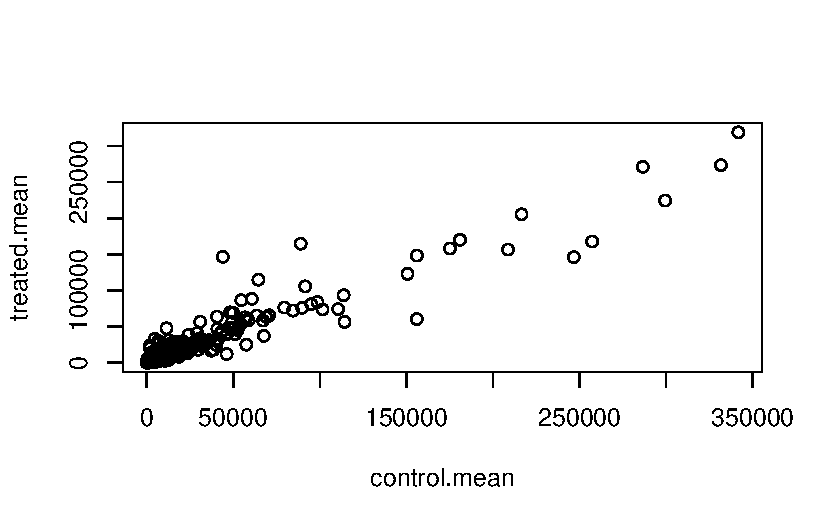
\includegraphics{Class13_files/figure-pdf/unnamed-chunk-13-1.pdf}

}

\end{figure}

\begin{quote}
• Q5 (b).You could also use the ggplot2 package to make this figure
producing the plot below. What geom\_?() function would you use for this
plot?
\end{quote}

\begin{Shaded}
\begin{Highlighting}[]
\FunctionTok{library}\NormalTok{(ggplot2)}

\FunctionTok{ggplot}\NormalTok{(meancounts) }\SpecialCharTok{+} 
  \FunctionTok{aes}\NormalTok{(control.mean, treated.mean) }\SpecialCharTok{+} 
  \FunctionTok{geom\_point}\NormalTok{(}\AttributeTok{alpha=}\FloatTok{0.2}\NormalTok{)}
\end{Highlighting}
\end{Shaded}

\begin{figure}[H]

{\centering 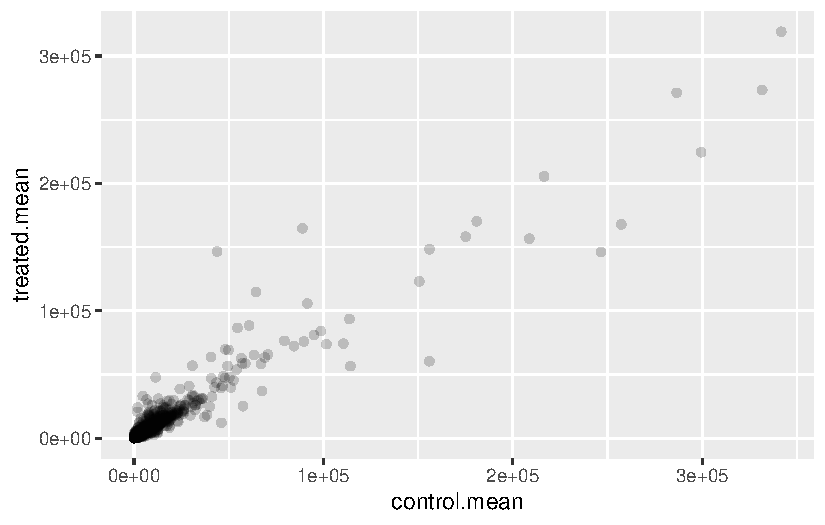
\includegraphics{Class13_files/figure-pdf/unnamed-chunk-14-1.pdf}

}

\end{figure}

\begin{quote}
Q6. Try plotting both axes on a log scale. What is the argument to
plot() that allows you to do this?
\end{quote}

\begin{Shaded}
\begin{Highlighting}[]
\FunctionTok{plot}\NormalTok{(meancounts, }\AttributeTok{log=}\StringTok{"xy"}\NormalTok{)}
\end{Highlighting}
\end{Shaded}

\begin{verbatim}
Warning in xy.coords(x, y, xlabel, ylabel, log): 15032 x values <= 0 omitted
from logarithmic plot
\end{verbatim}

\begin{verbatim}
Warning in xy.coords(x, y, xlabel, ylabel, log): 15281 y values <= 0 omitted
from logarithmic plot
\end{verbatim}

\begin{figure}[H]

{\centering 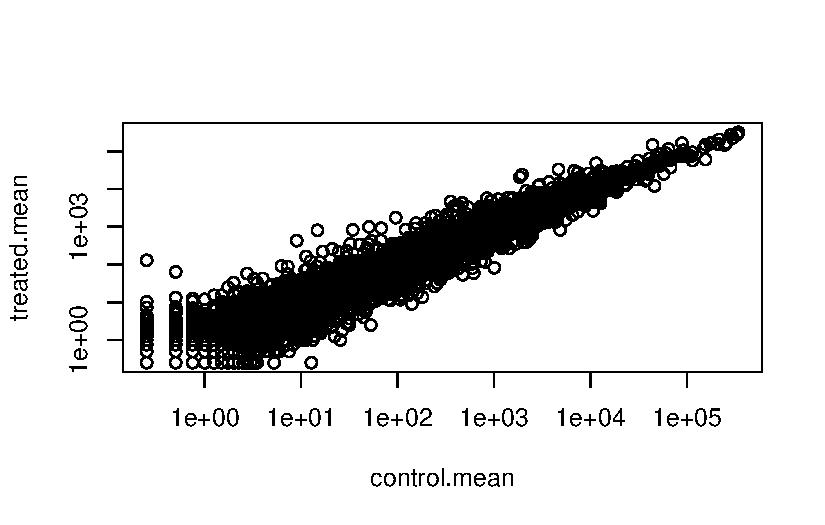
\includegraphics{Class13_files/figure-pdf/unnamed-chunk-15-1.pdf}

}

\end{figure}

Logs are useful when we have such skewed data.

\begin{Shaded}
\begin{Highlighting}[]
\CommentTok{\# Treated / control}

\FunctionTok{log2}\NormalTok{(}\DecValTok{10}\SpecialCharTok{/}\DecValTok{10}\NormalTok{)}
\end{Highlighting}
\end{Shaded}

\begin{verbatim}
[1] 0
\end{verbatim}

No change from treated vs control would show a 0 with log2. A doubling
in treated vs the control would show a 1 with log2.

Add log2(fold-change) values to our results table.

\begin{Shaded}
\begin{Highlighting}[]
\NormalTok{meancounts}\SpecialCharTok{$}\NormalTok{log2fc }\OtherTok{\textless{}{-}} \FunctionTok{log2}\NormalTok{(meancounts}\SpecialCharTok{$}\NormalTok{treated.mean}\SpecialCharTok{/}
\NormalTok{                            meancounts}\SpecialCharTok{$}\NormalTok{control.mean)}
\FunctionTok{head}\NormalTok{(meancounts)}
\end{Highlighting}
\end{Shaded}

\begin{verbatim}
                control.mean treated.mean      log2fc
ENSG00000000003       900.75       658.00 -0.45303916
ENSG00000000005         0.00         0.00         NaN
ENSG00000000419       520.50       546.00  0.06900279
ENSG00000000457       339.75       316.50 -0.10226805
ENSG00000000460        97.25        78.75 -0.30441833
ENSG00000000938         0.75         0.00        -Inf
\end{verbatim}

I need to exclude any genes with zero counts as we can't say anything
about them anyway from this experiment.

\begin{Shaded}
\begin{Highlighting}[]
\CommentTok{\# What values in the first two columns are zero?}
\NormalTok{to.rm.inds }\OtherTok{\textless{}{-}} \FunctionTok{rowSums}\NormalTok{(meancounts[,}\DecValTok{1}\SpecialCharTok{:}\DecValTok{2}\NormalTok{] }\SpecialCharTok{==} \DecValTok{0}\NormalTok{) }\SpecialCharTok{\textgreater{}} \DecValTok{0}
\DocumentationTok{\#\# print(to.rm.inds)}
\NormalTok{mycounts }\OtherTok{\textless{}{-}}\NormalTok{ meancounts[}\SpecialCharTok{!}\NormalTok{to.rm.inds, ]}
\end{Highlighting}
\end{Shaded}

\begin{quote}
Q. How many genes do I have left?
\end{quote}

\begin{Shaded}
\begin{Highlighting}[]
\FunctionTok{nrow}\NormalTok{(mycounts)}
\end{Highlighting}
\end{Shaded}

\begin{verbatim}
[1] 21817
\end{verbatim}

\begin{quote}
Q. How many genes are ``up regulated'' (i.e.~have a log2fold-change
greater than +2)
\end{quote}

\begin{Shaded}
\begin{Highlighting}[]
\FunctionTok{sum}\NormalTok{(mycounts}\SpecialCharTok{$}\NormalTok{log2fc }\SpecialCharTok{\textgreater{}} \SpecialCharTok{+}\DecValTok{2}\NormalTok{)}
\end{Highlighting}
\end{Shaded}

\begin{verbatim}
[1] 250
\end{verbatim}

\begin{quote}
Q. How many are ``down regulated''?
\end{quote}

\begin{Shaded}
\begin{Highlighting}[]
\FunctionTok{sum}\NormalTok{(mycounts}\SpecialCharTok{$}\NormalTok{log2fc }\SpecialCharTok{\textless{}} \SpecialCharTok{{-}}\DecValTok{2}\NormalTok{)}
\end{Highlighting}
\end{Shaded}

\begin{verbatim}
[1] 367
\end{verbatim}

\begin{quote}
Q7. What is the purpose of the arr.ind argument in the which() function
call above? Why would we then take the first column of the output and
need to call the unique() function?
\end{quote}

\hypertarget{running-deseq}{%
\subsection{Running DESeq}\label{running-deseq}}

Like many bioconductor analyssi packages, DESeq wants its input in a
very particular way.

\begin{Shaded}
\begin{Highlighting}[]
\NormalTok{dds }\OtherTok{\textless{}{-}} \FunctionTok{DESeqDataSetFromMatrix}\NormalTok{(}\AttributeTok{countData=}\NormalTok{counts,}
                              \AttributeTok{colData=}\NormalTok{metadata,}
                              \AttributeTok{design=}\SpecialCharTok{\textasciitilde{}}\NormalTok{dex)}
\end{Highlighting}
\end{Shaded}

\begin{verbatim}
converting counts to integer mode
\end{verbatim}

\begin{verbatim}
Warning in DESeqDataSet(se, design = design, ignoreRank): some variables in
design formula are characters, converting to factors
\end{verbatim}

To run DESeq analysis we call the main function from the package called
\texttt{DESeq(dds)}

\begin{Shaded}
\begin{Highlighting}[]
\NormalTok{dds }\OtherTok{\textless{}{-}} \FunctionTok{DESeq}\NormalTok{(dds)}
\end{Highlighting}
\end{Shaded}

\begin{verbatim}
estimating size factors
\end{verbatim}

\begin{verbatim}
estimating dispersions
\end{verbatim}

\begin{verbatim}
gene-wise dispersion estimates
\end{verbatim}

\begin{verbatim}
mean-dispersion relationship
\end{verbatim}

\begin{verbatim}
final dispersion estimates
\end{verbatim}

\begin{verbatim}
fitting model and testing
\end{verbatim}

To get the results back from this \texttt{dds} object, we can use the
DESeq \texttt{results()} function.

\begin{Shaded}
\begin{Highlighting}[]
\NormalTok{res }\OtherTok{\textless{}{-}} \FunctionTok{results}\NormalTok{(dds)}
\FunctionTok{head}\NormalTok{(res)}
\end{Highlighting}
\end{Shaded}

\begin{verbatim}
log2 fold change (MLE): dex treated vs control 
Wald test p-value: dex treated vs control 
DataFrame with 6 rows and 6 columns
                  baseMean log2FoldChange     lfcSE      stat    pvalue
                 <numeric>      <numeric> <numeric> <numeric> <numeric>
ENSG00000000003 747.194195     -0.3507030  0.168246 -2.084470 0.0371175
ENSG00000000005   0.000000             NA        NA        NA        NA
ENSG00000000419 520.134160      0.2061078  0.101059  2.039475 0.0414026
ENSG00000000457 322.664844      0.0245269  0.145145  0.168982 0.8658106
ENSG00000000460  87.682625     -0.1471420  0.257007 -0.572521 0.5669691
ENSG00000000938   0.319167     -1.7322890  3.493601 -0.495846 0.6200029
                     padj
                <numeric>
ENSG00000000003  0.163035
ENSG00000000005        NA
ENSG00000000419  0.176032
ENSG00000000457  0.961694
ENSG00000000460  0.815849
ENSG00000000938        NA
\end{verbatim}

A common summary visualization is called a Volcano Plot.

\begin{Shaded}
\begin{Highlighting}[]
\FunctionTok{plot}\NormalTok{(res}\SpecialCharTok{$}\NormalTok{log2FoldChange, }\SpecialCharTok{{-}}\FunctionTok{log}\NormalTok{(res}\SpecialCharTok{$}\NormalTok{padj),}
     \AttributeTok{xlab=}\StringTok{"Log2 Fold{-}Change"}\NormalTok{,}
     \AttributeTok{ylab=}\StringTok{"{-}log P{-}value"}\NormalTok{)}

\FunctionTok{abline}\NormalTok{(}\AttributeTok{v=}\FunctionTok{c}\NormalTok{(}\SpecialCharTok{{-}}\DecValTok{2}\NormalTok{,}\DecValTok{2}\NormalTok{), }\AttributeTok{col=}\StringTok{"red"}\NormalTok{)}
\FunctionTok{abline}\NormalTok{(}\AttributeTok{h=}\SpecialCharTok{{-}}\FunctionTok{log}\NormalTok{(}\FloatTok{0.05}\NormalTok{), }\AttributeTok{col=}\StringTok{"blue"}\NormalTok{)}
\end{Highlighting}
\end{Shaded}

\begin{figure}[H]

{\centering 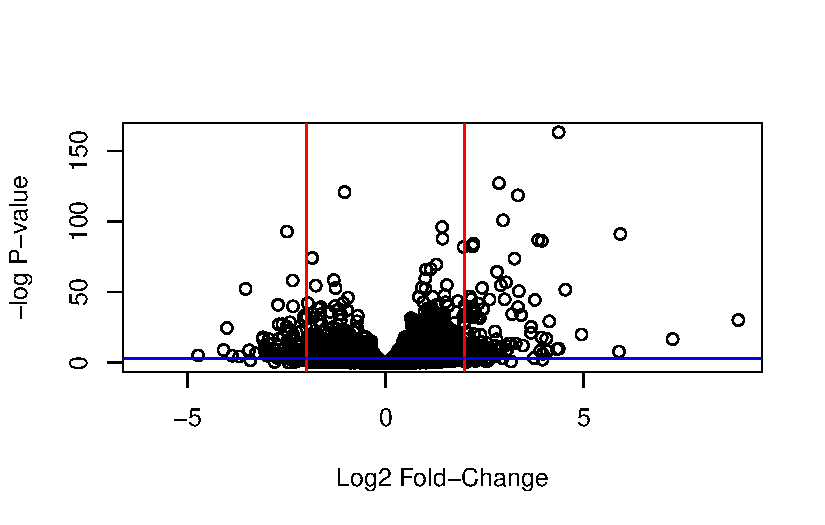
\includegraphics{Class13_files/figure-pdf/unnamed-chunk-25-1.pdf}

}

\end{figure}

\begin{Shaded}
\begin{Highlighting}[]
\NormalTok{mycols }\OtherTok{\textless{}{-}} \FunctionTok{rep}\NormalTok{(}\StringTok{"grey"}\NormalTok{, }\FunctionTok{nrow}\NormalTok{(res))}
\NormalTok{mycols[ res}\SpecialCharTok{$}\NormalTok{log2FoldChange }\SpecialCharTok{\textgreater{}} \DecValTok{2}\NormalTok{ ] }\OtherTok{\textless{}{-}} \StringTok{"black"}
\NormalTok{mycols[ res}\SpecialCharTok{$}\NormalTok{log2FoldChange }\SpecialCharTok{\textless{}} \SpecialCharTok{{-}}\DecValTok{2}\NormalTok{ ] }\OtherTok{\textless{}{-}} \StringTok{"black"}
\NormalTok{mycols[ res}\SpecialCharTok{$}\NormalTok{padj }\SpecialCharTok{\textgreater{}} \FloatTok{0.05}\NormalTok{ ] }\OtherTok{\textless{}{-}} \StringTok{"grey"}
\end{Highlighting}
\end{Shaded}

\begin{Shaded}
\begin{Highlighting}[]
\FunctionTok{plot}\NormalTok{(res}\SpecialCharTok{$}\NormalTok{log2FoldChange, }\SpecialCharTok{{-}}\FunctionTok{log}\NormalTok{(res}\SpecialCharTok{$}\NormalTok{padj), }\AttributeTok{col=}\NormalTok{mycols,}
     \AttributeTok{xlab=}\StringTok{"Log2 Fold{-}Change"}\NormalTok{,}
     \AttributeTok{ylab=}\StringTok{"{-}log P{-}value"}\NormalTok{)}

\FunctionTok{abline}\NormalTok{(}\AttributeTok{v=}\FunctionTok{c}\NormalTok{(}\SpecialCharTok{{-}}\DecValTok{2}\NormalTok{,}\DecValTok{2}\NormalTok{), }\AttributeTok{col=}\StringTok{"red"}\NormalTok{)}
\FunctionTok{abline}\NormalTok{(}\AttributeTok{h=}\SpecialCharTok{{-}}\FunctionTok{log}\NormalTok{(}\FloatTok{0.05}\NormalTok{), }\AttributeTok{col=}\StringTok{"blue"}\NormalTok{)}
\end{Highlighting}
\end{Shaded}

\begin{figure}[H]

{\centering 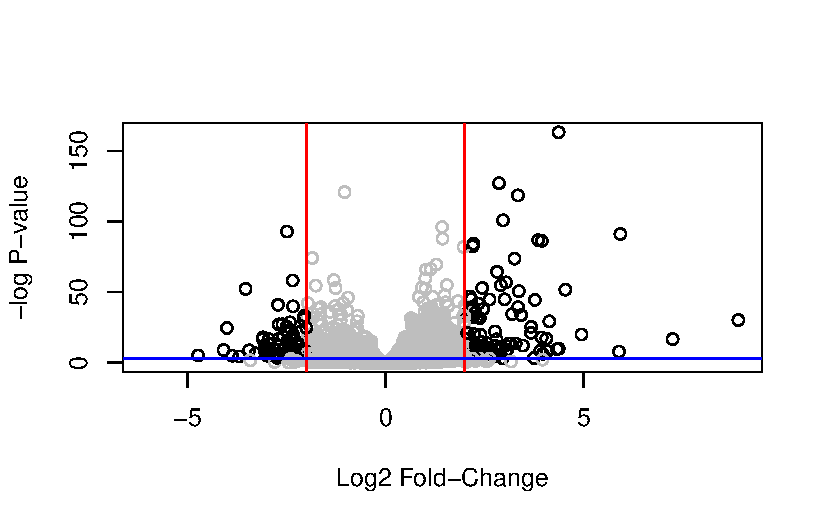
\includegraphics{Class13_files/figure-pdf/unnamed-chunk-27-1.pdf}

}

\end{figure}

\hypertarget{save-our-results-to-date}{%
\section{Save our results to date}\label{save-our-results-to-date}}

\begin{Shaded}
\begin{Highlighting}[]
\FunctionTok{write.csv}\NormalTok{(res, }\AttributeTok{file=}\StringTok{"myresults.csv"}\NormalTok{)}
\end{Highlighting}
\end{Shaded}

\hypertarget{adding-annotation-data}{%
\section{Adding annotation data}\label{adding-annotation-data}}

We need to translate or ``map'' our ensemble IDs into more
understandable gene names and identifiers that other useful databases
have. (We will use the mapID function)

\begin{Shaded}
\begin{Highlighting}[]
\FunctionTok{library}\NormalTok{(}\StringTok{"AnnotationDbi"}\NormalTok{)}
\FunctionTok{library}\NormalTok{(}\StringTok{"org.Hs.eg.db"}\NormalTok{)}
\end{Highlighting}
\end{Shaded}

\begin{verbatim}
\end{verbatim}

\begin{Shaded}
\begin{Highlighting}[]
\FunctionTok{columns}\NormalTok{(org.Hs.eg.db)}
\end{Highlighting}
\end{Shaded}

\begin{verbatim}
 [1] "ACCNUM"       "ALIAS"        "ENSEMBL"      "ENSEMBLPROT"  "ENSEMBLTRANS"
 [6] "ENTREZID"     "ENZYME"       "EVIDENCE"     "EVIDENCEALL"  "GENENAME"    
[11] "GENETYPE"     "GO"           "GOALL"        "IPI"          "MAP"         
[16] "OMIM"         "ONTOLOGY"     "ONTOLOGYALL"  "PATH"         "PFAM"        
[21] "PMID"         "PROSITE"      "REFSEQ"       "SYMBOL"       "UCSCKG"      
[26] "UNIPROT"     
\end{verbatim}

\begin{Shaded}
\begin{Highlighting}[]
\NormalTok{ res}\SpecialCharTok{$}\NormalTok{symbol }\OtherTok{\textless{}{-}} \FunctionTok{mapIds}\NormalTok{(org.Hs.eg.db,}
                        \AttributeTok{keys=}\FunctionTok{row.names}\NormalTok{(res), }\CommentTok{\# Our genenames}
                        \AttributeTok{keytype=}\StringTok{"ENSEMBL"}\NormalTok{, }\CommentTok{\# The format of our genenames}
                        \AttributeTok{column=}\StringTok{"SYMBOL"}\NormalTok{, }\CommentTok{\# The new format we want to add}
                        \AttributeTok{multiVals=}\StringTok{"first"}\NormalTok{)}
\end{Highlighting}
\end{Shaded}

\begin{verbatim}
'select()' returned 1:many mapping between keys and columns
\end{verbatim}

\begin{Shaded}
\begin{Highlighting}[]
\FunctionTok{head}\NormalTok{(res)}
\end{Highlighting}
\end{Shaded}

\begin{verbatim}
log2 fold change (MLE): dex treated vs control 
Wald test p-value: dex treated vs control 
DataFrame with 6 rows and 7 columns
                  baseMean log2FoldChange     lfcSE      stat    pvalue
                 <numeric>      <numeric> <numeric> <numeric> <numeric>
ENSG00000000003 747.194195     -0.3507030  0.168246 -2.084470 0.0371175
ENSG00000000005   0.000000             NA        NA        NA        NA
ENSG00000000419 520.134160      0.2061078  0.101059  2.039475 0.0414026
ENSG00000000457 322.664844      0.0245269  0.145145  0.168982 0.8658106
ENSG00000000460  87.682625     -0.1471420  0.257007 -0.572521 0.5669691
ENSG00000000938   0.319167     -1.7322890  3.493601 -0.495846 0.6200029
                     padj      symbol
                <numeric> <character>
ENSG00000000003  0.163035      TSPAN6
ENSG00000000005        NA        TNMD
ENSG00000000419  0.176032        DPM1
ENSG00000000457  0.961694       SCYL3
ENSG00000000460  0.815849       FIRRM
ENSG00000000938        NA         FGR
\end{verbatim}

\begin{quote}
Q11. Run the mapIds() function two more times to add the Entrez ID and
UniProt accession and GENENAME as new columns called
res\(entrez, res\)uniprot and res\$genename.
\end{quote}

\begin{Shaded}
\begin{Highlighting}[]
\NormalTok{res}\SpecialCharTok{$}\NormalTok{entrez }\OtherTok{\textless{}{-}} \FunctionTok{mapIds}\NormalTok{(org.Hs.eg.db,}
                        \AttributeTok{keys=}\FunctionTok{row.names}\NormalTok{(res), }\CommentTok{\# Our genenames}
                        \AttributeTok{keytype=}\StringTok{"ENSEMBL"}\NormalTok{, }\CommentTok{\# The format of our genenames}
                        \AttributeTok{column=}\StringTok{"ENTREZID"}\NormalTok{, }\CommentTok{\# The new format we want to add}
                        \AttributeTok{multiVals=}\StringTok{"first"}\NormalTok{)}
\end{Highlighting}
\end{Shaded}

\begin{verbatim}
'select()' returned 1:many mapping between keys and columns
\end{verbatim}

\begin{Shaded}
\begin{Highlighting}[]
\FunctionTok{head}\NormalTok{(res)}
\end{Highlighting}
\end{Shaded}

\begin{verbatim}
log2 fold change (MLE): dex treated vs control 
Wald test p-value: dex treated vs control 
DataFrame with 6 rows and 8 columns
                  baseMean log2FoldChange     lfcSE      stat    pvalue
                 <numeric>      <numeric> <numeric> <numeric> <numeric>
ENSG00000000003 747.194195     -0.3507030  0.168246 -2.084470 0.0371175
ENSG00000000005   0.000000             NA        NA        NA        NA
ENSG00000000419 520.134160      0.2061078  0.101059  2.039475 0.0414026
ENSG00000000457 322.664844      0.0245269  0.145145  0.168982 0.8658106
ENSG00000000460  87.682625     -0.1471420  0.257007 -0.572521 0.5669691
ENSG00000000938   0.319167     -1.7322890  3.493601 -0.495846 0.6200029
                     padj      symbol      entrez
                <numeric> <character> <character>
ENSG00000000003  0.163035      TSPAN6        7105
ENSG00000000005        NA        TNMD       64102
ENSG00000000419  0.176032        DPM1        8813
ENSG00000000457  0.961694       SCYL3       57147
ENSG00000000460  0.815849       FIRRM       55732
ENSG00000000938        NA         FGR        2268
\end{verbatim}

\begin{Shaded}
\begin{Highlighting}[]
\NormalTok{res}\SpecialCharTok{$}\NormalTok{uniprot }\OtherTok{\textless{}{-}} \FunctionTok{mapIds}\NormalTok{(org.Hs.eg.db,}
                        \AttributeTok{keys=}\FunctionTok{row.names}\NormalTok{(res), }\CommentTok{\# Our genenames}
                        \AttributeTok{keytype=}\StringTok{"ENSEMBL"}\NormalTok{, }\CommentTok{\# The format of our genenames}
                        \AttributeTok{column=}\StringTok{"UNIPROT"}\NormalTok{, }\CommentTok{\# The new format we want to add}
                        \AttributeTok{multiVals=}\StringTok{"first"}\NormalTok{)}
\end{Highlighting}
\end{Shaded}

\begin{verbatim}
'select()' returned 1:many mapping between keys and columns
\end{verbatim}

\begin{Shaded}
\begin{Highlighting}[]
\FunctionTok{head}\NormalTok{(res)}
\end{Highlighting}
\end{Shaded}

\begin{verbatim}
log2 fold change (MLE): dex treated vs control 
Wald test p-value: dex treated vs control 
DataFrame with 6 rows and 9 columns
                  baseMean log2FoldChange     lfcSE      stat    pvalue
                 <numeric>      <numeric> <numeric> <numeric> <numeric>
ENSG00000000003 747.194195     -0.3507030  0.168246 -2.084470 0.0371175
ENSG00000000005   0.000000             NA        NA        NA        NA
ENSG00000000419 520.134160      0.2061078  0.101059  2.039475 0.0414026
ENSG00000000457 322.664844      0.0245269  0.145145  0.168982 0.8658106
ENSG00000000460  87.682625     -0.1471420  0.257007 -0.572521 0.5669691
ENSG00000000938   0.319167     -1.7322890  3.493601 -0.495846 0.6200029
                     padj      symbol      entrez     uniprot
                <numeric> <character> <character> <character>
ENSG00000000003  0.163035      TSPAN6        7105  A0A024RCI0
ENSG00000000005        NA        TNMD       64102      Q9H2S6
ENSG00000000419  0.176032        DPM1        8813      O60762
ENSG00000000457  0.961694       SCYL3       57147      Q8IZE3
ENSG00000000460  0.815849       FIRRM       55732  A0A024R922
ENSG00000000938        NA         FGR        2268      P09769
\end{verbatim}

\begin{Shaded}
\begin{Highlighting}[]
\NormalTok{res}\SpecialCharTok{$}\NormalTok{genename }\OtherTok{\textless{}{-}} \FunctionTok{mapIds}\NormalTok{(org.Hs.eg.db,}
                        \AttributeTok{keys=}\FunctionTok{row.names}\NormalTok{(res), }\CommentTok{\# Our genenames}
                        \AttributeTok{keytype=}\StringTok{"ENSEMBL"}\NormalTok{, }\CommentTok{\# The format of our genenames}
                        \AttributeTok{column=}\StringTok{"GENENAME"}\NormalTok{, }\CommentTok{\# The new format we want to add}
                        \AttributeTok{multiVals=}\StringTok{"first"}\NormalTok{)}
\end{Highlighting}
\end{Shaded}

\begin{verbatim}
'select()' returned 1:many mapping between keys and columns
\end{verbatim}

\begin{Shaded}
\begin{Highlighting}[]
\FunctionTok{head}\NormalTok{(res)}
\end{Highlighting}
\end{Shaded}

\begin{verbatim}
log2 fold change (MLE): dex treated vs control 
Wald test p-value: dex treated vs control 
DataFrame with 6 rows and 10 columns
                  baseMean log2FoldChange     lfcSE      stat    pvalue
                 <numeric>      <numeric> <numeric> <numeric> <numeric>
ENSG00000000003 747.194195     -0.3507030  0.168246 -2.084470 0.0371175
ENSG00000000005   0.000000             NA        NA        NA        NA
ENSG00000000419 520.134160      0.2061078  0.101059  2.039475 0.0414026
ENSG00000000457 322.664844      0.0245269  0.145145  0.168982 0.8658106
ENSG00000000460  87.682625     -0.1471420  0.257007 -0.572521 0.5669691
ENSG00000000938   0.319167     -1.7322890  3.493601 -0.495846 0.6200029
                     padj      symbol      entrez     uniprot
                <numeric> <character> <character> <character>
ENSG00000000003  0.163035      TSPAN6        7105  A0A024RCI0
ENSG00000000005        NA        TNMD       64102      Q9H2S6
ENSG00000000419  0.176032        DPM1        8813      O60762
ENSG00000000457  0.961694       SCYL3       57147      Q8IZE3
ENSG00000000460  0.815849       FIRRM       55732  A0A024R922
ENSG00000000938        NA         FGR        2268      P09769
                              genename
                           <character>
ENSG00000000003          tetraspanin 6
ENSG00000000005            tenomodulin
ENSG00000000419 dolichyl-phosphate m..
ENSG00000000457 SCY1 like pseudokina..
ENSG00000000460 FIGNL1 interacting r..
ENSG00000000938 FGR proto-oncogene, ..
\end{verbatim}

\hypertarget{pathway-analysis}{%
\section{Pathway analysis}\label{pathway-analysis}}

\begin{Shaded}
\begin{Highlighting}[]
 \FunctionTok{library}\NormalTok{(pathview)}
\end{Highlighting}
\end{Shaded}

\begin{verbatim}
##############################################################################
Pathview is an open source software package distributed under GNU General
Public License version 3 (GPLv3). Details of GPLv3 is available at
http://www.gnu.org/licenses/gpl-3.0.html. Particullary, users are required to
formally cite the original Pathview paper (not just mention it) in publications
or products. For details, do citation("pathview") within R.

The pathview downloads and uses KEGG data. Non-academic uses may require a KEGG
license agreement (details at http://www.kegg.jp/kegg/legal.html).
##############################################################################
\end{verbatim}

\begin{Shaded}
\begin{Highlighting}[]
   \FunctionTok{library}\NormalTok{(gage)}
\end{Highlighting}
\end{Shaded}

\begin{verbatim}
\end{verbatim}

\begin{Shaded}
\begin{Highlighting}[]
   \FunctionTok{library}\NormalTok{(gageData)}
   \FunctionTok{data}\NormalTok{(kegg.sets.hs)}
   \CommentTok{\# Examine the first 2 pathways in this kegg set for humans}
   \FunctionTok{head}\NormalTok{(kegg.sets.hs, }\DecValTok{2}\NormalTok{)}
\end{Highlighting}
\end{Shaded}

\begin{verbatim}
$`hsa00232 Caffeine metabolism`
[1] "10"   "1544" "1548" "1549" "1553" "7498" "9"   

$`hsa00983 Drug metabolism - other enzymes`
 [1] "10"     "1066"   "10720"  "10941"  "151531" "1548"   "1549"   "1551"  
 [9] "1553"   "1576"   "1577"   "1806"   "1807"   "1890"   "221223" "2990"  
[17] "3251"   "3614"   "3615"   "3704"   "51733"  "54490"  "54575"  "54576" 
[25] "54577"  "54578"  "54579"  "54600"  "54657"  "54658"  "54659"  "54963" 
[33] "574537" "64816"  "7083"   "7084"   "7172"   "7363"   "7364"   "7365"  
[41] "7366"   "7367"   "7371"   "7372"   "7378"   "7498"   "79799"  "83549" 
[49] "8824"   "8833"   "9"      "978"   
\end{verbatim}

\begin{Shaded}
\begin{Highlighting}[]
\NormalTok{foldchanges }\OtherTok{=}\NormalTok{ res}\SpecialCharTok{$}\NormalTok{log2FoldChange}
\FunctionTok{names}\NormalTok{(foldchanges) }\OtherTok{=}\NormalTok{ res}\SpecialCharTok{$}\NormalTok{entrez}
\FunctionTok{head}\NormalTok{(foldchanges)}
\end{Highlighting}
\end{Shaded}

\begin{verbatim}
       7105       64102        8813       57147       55732        2268 
-0.35070302          NA  0.20610777  0.02452695 -0.14714205 -1.73228897 
\end{verbatim}

Run gage:

\begin{Shaded}
\begin{Highlighting}[]
\CommentTok{\# Get the results}
\NormalTok{keggres }\OtherTok{=} \FunctionTok{gage}\NormalTok{(foldchanges, }\AttributeTok{gsets=}\NormalTok{kegg.sets.hs)}
\end{Highlighting}
\end{Shaded}

\begin{Shaded}
\begin{Highlighting}[]
\FunctionTok{attributes}\NormalTok{(keggres)}
\end{Highlighting}
\end{Shaded}

\begin{verbatim}
$names
[1] "greater" "less"    "stats"  
\end{verbatim}

\begin{Shaded}
\begin{Highlighting}[]
\CommentTok{\# Look at the first 3 down (less) pathways}
\FunctionTok{head}\NormalTok{(keggres}\SpecialCharTok{$}\NormalTok{less, }\DecValTok{3}\NormalTok{)}
\end{Highlighting}
\end{Shaded}

\begin{verbatim}
                                      p.geomean stat.mean        p.val
hsa05332 Graft-versus-host disease 0.0004250461 -3.473346 0.0004250461
hsa04940 Type I diabetes mellitus  0.0017820293 -3.002352 0.0017820293
hsa05310 Asthma                    0.0020045888 -3.009050 0.0020045888
                                        q.val set.size         exp1
hsa05332 Graft-versus-host disease 0.09053483       40 0.0004250461
hsa04940 Type I diabetes mellitus  0.14232581       42 0.0017820293
hsa05310 Asthma                    0.14232581       29 0.0020045888
\end{verbatim}

Let's have a look at one of these pathways

\begin{Shaded}
\begin{Highlighting}[]
\FunctionTok{pathview}\NormalTok{(}\AttributeTok{gene.data=}\NormalTok{foldchanges, }\AttributeTok{pathway.id=}\StringTok{"hsa05310"}\NormalTok{)}
\end{Highlighting}
\end{Shaded}

\begin{verbatim}
'select()' returned 1:1 mapping between keys and columns
\end{verbatim}

\begin{verbatim}
Info: Working in directory /Users/andybellaart/Desktop/BGGN213/Class13
\end{verbatim}

\begin{verbatim}
Info: Writing image file hsa05310.pathview.png
\end{verbatim}

\includegraphics{hsa03510.pathview.png}



\end{document}
